%%% LaTeX Template: Article/Thesis/etc. with colored headings and special fonts
%%%
%%% Source: http://www.howtotex.com/
%%% Feel free to distribute this template, but please keep to referal to http://www.howtotex.com/ here.
%%% February 2011
%%%
%%% Modified May 2018 by CDM

%%%  Preamble
\documentclass[11pt,letterpaper]{article}
\usepackage[margin=1.0in]{geometry}
\usepackage[T1]{fontenc}
\usepackage[bitstream-charter]{mathdesign}
\usepackage[latin1]{inputenc}					
\usepackage{amsmath}						
\usepackage{xcolor}
\usepackage{cite}
\usepackage{hyphenat}
\usepackage{graphicx}
\usepackage{float}
\usepackage{subfigure}
\usepackage{sectsty}
\usepackage[compact]{titlesec} 
\usepackage[tablegrid]{vhistory}
\allsectionsfont{\color{accentcolor}\scshape\selectfont}

%%% Definitions
\definecolor{accentcolor}{rgb}{0.0,0.0,0.5} 
\newcommand{\teamname}{Team UR5}
\newcommand{\productname}{Checkers-Playing UR5 Co-bot}
\newcommand{\coursename}{CSE 4316: Senior Design I}
\newcommand{\semester}{Fall 2022}
\newcommand{\docname}{System Requirements Specification}
\newcommand{\department}{Department of Computer Science \& Engineering}
\newcommand{\university}{The University of Texas at Arlington}
\newcommand{\authors}{Nimita Uprety \\ Patricia Rojas \\ Hoang Ho \\ Kevin Vu \\ Joanna Huynh}
%%% Headers and footers
\usepackage{fancyhdr}
	\pagestyle{fancy}						% Enabling the custom headers/footers
\usepackage{lastpage}	
	% Header (empty)
	\lhead{}
	\chead{}
	\rhead{}
	% Footer
	\lfoot{\footnotesize \teamname \ - \semester}
	\cfoot{}
	\rfoot{\footnotesize page \thepage\ of \pageref{LastPage}}	% "Page 1 of 2"
	\renewcommand{\headrulewidth}{0.0pt}
	\renewcommand{\footrulewidth}{0.4pt}

%%% Change the abstract environment
\usepackage[runin]{abstract}			% runin option for a run-in title
%\setlength\absleftindent{30pt}			% left margin
%\setlength\absrightindent{30pt}		% right margin
\abslabeldelim{\quad}	
\setlength{\abstitleskip}{-10pt}
\renewcommand{\abstractname}{}
\renewcommand{\abstracttextfont}{\color{accentcolor} \small \slshape}	% slanted text

%%% Start of the document
\begin{document}

%%% Cover sheet
{\centering \huge \color{accentcolor} \sc \textbf{\department \\ \university} \par}
\vspace{1 in}
{\centering \huge \color{accentcolor} \sc \textbf{\docname \\ \coursename \\ \semester} \par}
% \vspace{0.5 in}
\begin{figure}[h!]
	\centering
   	
\includegraphics[width=0.60\textwidth]{images/Draft-Logo.png}
\end{figure}
% \vspace{0.5 in}
{\centering \huge \color{accentcolor} \sc \textbf{\teamname \\ \productname} \par}
\vspace{0.25 in}
{\centering \large \sc \textbf{\authors} \par}
\newpage


%\vspace{1 in}
%\centerline{January 13th, 2012}
%\newpage

%%% Revision History
\begin{versionhistory}
  	\vhEntry{0.1}{10.05.2022}{HH}{document creation}
  	\vhEntry{0.2}{10.23.2022}{NU|HH|PR|KV|JH}{complete draft}
%   	\vhEntry{0.3}{10.12.2015}{AT|GH}{release candidate 1}
  	\vhEntry{1.0}{10.24.2022}{NU|HH|PR|KV|JH}{official release}
    \vhEntry{1.1}{05.09.2023}{NU}{final revisions}
    \vhEntry{1.2}{05.10.2023}{NU|HH|PR|KV|JH}{final revisions}
\end{versionhistory}
\newpage

%%% Table of contents
\setcounter{tocdepth}{3}
\tableofcontents
\newpage

%%% List of figures and tables (optional)
\listoffigures
%\listoftables
\newpage

\section{Product Concept}
% This section provides a high-level statement of your product concept - what it is intended to do and how it is intended to be used. Include in this header paragraph, a brief synopsis of what is described here. For example, this header paragraph might say something like: "This section describes the purpose, use and intended user audience for the X product. X is a system that performs Y. Users of X will be able to Z..."

This section describes the purpose, use \& intended audience for our programmed UR5 collaborative robot (co-bot). The UR5 co-bot will be programmed to be able to play the interactive \& strategy-based game, checkers, against a human opponent. The robot will have an electropermanent magnetic attachment that will allow it to pick up and move the individual checkers pieces. The robot is not intended to beat the human opponent every time but rather just have the ability to play a full game of checkers against them.

\subsection{Purpose and Use}
% This is where you describe in a brief, yet clear and concise, manner what your product should do and how you expect it should be used.

Our project aims to showcase the UR5 co-bot's abilities as a means of promoting the UT Arlington College of Engineering to prospective students through the means of an interactive demonstration. Students visiting the College of Engineering are expected to be able to engage with the product in a game of checkers, which will provide the potential Mavericks with an enjoyable and educational experience.

\subsection{Intended Audience}
% This is where you describe the intended audience(s) of your product. If this product were to be made available publicly or commercially, who would purchase or use it? Is the product designed for a particular customer, or an overall class of customers? Is it intended for general use, or is it a specific component of a more complex system?

The intended audience of our product is the UT Arlington College of Engineering, Department of Computer Science \& Engineering as well as the university as a whole to utilize the co-bot as a marketing strategy for prospective students. If this product were to be made commercially available it would be feasible and our primary customers would be other universities aiming to also recruit future engineers. Although the UR5 co-bot is intended to be operated by a student or faculty member of the university, the end user is a member of the public as the project is intended for general use.

\begin{figure}[h!]
	\centering
   	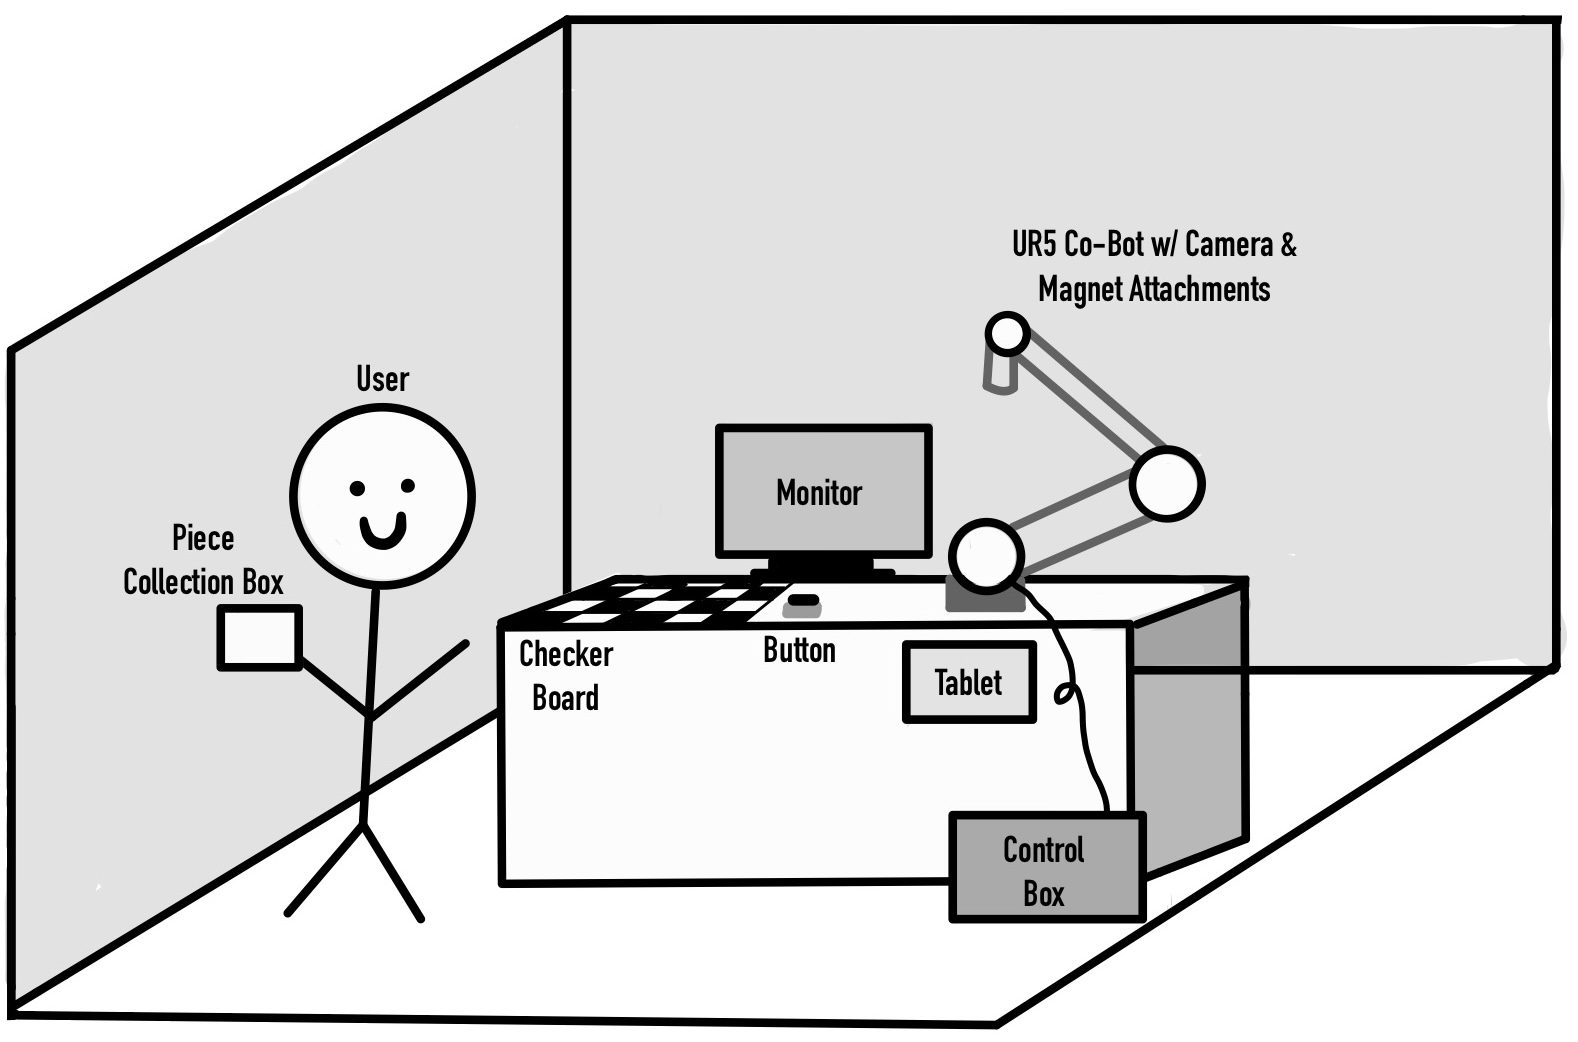
\includegraphics[width=0.90\textwidth]{images/Conceptual-Drawing.jpg}
    \caption{Conceptual Drawing}
\end{figure}

\newpage
\section{Product Description}
% This section provides a description of your product and defines it's primary features and functions. The purpose is to give the document reader/reviewer enough information about the product to allow them to easily follow the specification of requirements found in the remainder of the document. Your header for this section should introduce the section with a brief statement such as: "This section provides the reader with an overview of X. The primary operational aspects of the product, from the perspective of end users, maintainers and administrators, are defined here. The key features and functions found in the product, as well as critical user interactions and user interfaces are described in detail." Using words, and pictures or graphics where possible, specify the following:

This section provides the reader with an overview of our Checkers-Playing UR5 Co-Bot product. The primary operational aspects of the product from the perspective of end users \& maintainers, are defined here. The key features \& functions found in the product, as well as critical user interactions are described in detail.

\subsection{Features \& Functions}
% What the product does and does not do. Specify in words what it looks like, referring to a conceptual diagram/graphic (Figure X).  Define the principle parts/components of the product. Specify the elements in the diagram/graphic that are part(s) of this product as well as any associated external elements (e.g., the Internet, an external web server, a GPS satellite, etc.)
Our programmed UR5 co-bot is intended to have the following features and functions as outlined in Figure 1:
\begin{itemize}
  \item UR5 Robot Arm: core element of the product that is a programmable Universal Robots Arm with a 5 kg payload.
  \begin{itemize}
      \item Camera: 3D camera that will be mounted to a tall tripod to view the board and analyze it.
      \item Electropermanent Magnet Attachment: will allow the robot arm to pick up pieces individually by turning on the magnet \& then place the pieces by turning off the magnet.
  \end{itemize}
  \item Checker Board \& Pieces: these game pieces will be fundamental to the product as they are what will allow the game-play between the UR5 bot and human user to take place.
  \item Tablet: UR+ Teach Pendant device that will be used to control the robot step by step
  \item Control Box: OEM Control Box that not only powers the UR5 co-bot but also allows for integration with external devices.
  \item Keyboard: Input from the keyboard that will allow the user to notify the robot when they have completed their turn.
  \item Piece Collection Box: Would ideally sit on the table next the the checkers board to allow both the human user and the co-bot to place pieces they have "won".
  \item Monitor: Will display the computerized version of the current state of the board.
\end{itemize}

\subsection{External Inputs \& Outputs}
% Describe critical external data flows. What does your product require/expect to receive from end users or external systems (inputs), and what is expected to be created by your product for consumption by end users or external systems (outputs)? In other words, specify here all data/information to flow into and out of your systems. A table works best here, with rows for each critical data element, and columns for name, description and use.
Given the nature of our project there is only a single external data flow. Our UR5 Co-bot is expected to receive input from end users via the keyboard input that they will press upon completion of their turn, thus signalling the robot to play their next move.

\subsection{Product Interfaces}
% Specify what all operational (visible) interfaces look like to your end-user, administrator, maintainer, etc. Show sample/mocked-up screen shots, graphics of buttons, panels, etc. Refer to the critical external inputs and outputs described in the paragraph above.

Our product will have a simple computerized version this is intended to show the current location of each players pieces.
\newpage
\section{Customer Requirements}
% Include a header paragraph specific to your product here. Customer requirements are those required features and functions specified for and by the intended audience for this product. This section establishes, clearly and concisely, the "look and feel" of the product, what each potential end-user should expect the product do and/or not do. Each requirement specified in this section is associated with a specific customer need that will be satisfied. In general Customer Requirements are the directly observable features and functions of the product that will be encountered by its users. Requirements specified in this section are created with, and must not be changed without, specific agreement of the intended customer/user/sponsor.

% \subsection{Requirement Name}
% \subsubsection{Description}
% A detailed description of the feature/function that satisfies the requirement. For example: \textit{The GUI background will be slate blue. This specific color is required in order to ensure that the GUI matches other similar software products offered by the customer. Slate blue is specified as \#007FFF, using six-digit hexadecimal color specification.} It is acceptable and advisable to include drawings/graphics in the description if it aids understanding of the requirement.
% \subsubsection{Source}
% The source of the requirement (e.g. customer, sponsor, specified team member (by name), federal regulation, local laws, CSE Senior Design project specifications, etc.)
% \subsubsection{Constraints}
% A detailed description of realistic constraints relevant to this requirement. Economic, environmental, social, political, ethical, health \& safety, manufacturability, and sustainability should be discussed as appropriate.
% \subsubsection{Standards}
% A detailed description of any specific standards that apply to this requirement (e.g. \textit{NSTM standard xx.xxx.x. color specifications \cite{Rubin2012}}. Standards exist for practically everything (ATC standard fuses, IEEE 802.15.4 embedded wireless, TLS 1.3 encryption, etc.), so be sure that you research and document which ones will be followed in meeting this requirement.
% \subsubsection{Priority}
% The priority of this requirement relative to other specified requirements. Use the following priorities:
% \begin{itemize}
% \item Critical (must have or product is a failure)
% \item High (very important to customer acceptance, desirability)
% \item Moderate (should have for proper product functionality);
% \item Low (nice to have, will include if time/resource permits)
% \item Future (not feasible in this version of the product, but should be considered for a future release).
% \end{itemize}

% \subsection{Requirement Name}
% \subsubsection{Description}
% Detailed requirement description...
% \subsubsection{Source}
% Source
% \subsubsection{Constraints}
% Detailed description of applicable constraints...
% \subsubsection{Standards}
% List of applicable standards
% \subsubsection{Priority}
% Priority

The customers of the UR5 Checkers-Playing Co-bot include, but are not limited to, the project sponsor, the developers, peers, UTA College of Engineering, and prospective students. This section establishes what the end-user should expect with the product. The co-bot will come with a custom-made checkerboard and custom-made checkers pieces to ensure that the physical components of the game are large enough to be detected by the UR5 co-bot's magnetic electro-permanent gripper. The product will also include a collection box for both the user and robot to deposit the checkers pieces during the match. The user will have control over terminating or resetting the match.   

\subsection{The product shall have a custom-made checkerboard.}
\subsubsection{Description}
The checkerboard will be constructed of a 18 inch by 18 inch wooden board and be custom-painted. It is custom-made to ensure that the size of the checkerboard and checkers pieces are large enough to be easily detected and grasped by the robot arm.
\subsubsection{Source}
Kevin Vu
\subsubsection{Constraints}
The custom board must be small enough to comfortably fit the UR5 stand base, and the squares must be large enough to fit the checkers pieces.
\subsubsection{Standards}
N/A
\subsubsection{Priority}
Critical

\subsection{The product shall have custom-made checker pieces.}
\subsubsection{Description}
These checker pieces will be 3D printed and will have a small magnet contained within them for the robot to grip the piece.
\subsubsection{Source}
Hoang Ho
\subsubsection{Constraints}
The checker pieces need to have a hole cut out for the washers to be inserted in them for easy pickup by the magnet in the robot arm. 
\subsubsection{Standards}
N/A
\subsubsection{Priority}
Critical

\subsection{The product shall have a piece collection box.}
\subsubsection{Description}
The box will hold the checkers pieces that the robot arm picks up throughout a checkers match. Additionally, when storing away the game, the checkers pieces can go in here.
\subsubsection{Source}
Kevin Vu
\subsubsection{Constraints}
The box must be in reach of the UR5 robot arm during game play to drop off its checker pieces.
\subsubsection{Standards}
N/A
\subsubsection{Priority}
High

\subsection{The UR5 robot arm shall have a magnetic electro-permanent gripper.}
\subsubsection{Description}
This gripper will have the ability to turn on to grip, and turn off to ungrip. The gripper will be used by the robot arm to pick up checker pieces, and make its move.
\subsubsection{Source}
Hoang Ho
\subsubsection{Constraints}
Objects may need to have certain magnetic strength to be able to be picked up by the gripper. On the other hand, the gripper magnetic strength may be needed to take into account also, so that checker pieces relative to the one the robot arm is picking up is not picked up either. It may be that we may need to use a different type of gripper for the optimal object pick up motion. We may be limited by the different magnets we can buy whether it be size, strength, or budget. These limitations also apply to the gripper itself.
\subsubsection{Standards}
N/A
\subsubsection{Priority}
Critical

\subsection{The system shall follow the rules of American checkers.}
\subsection{Description}
The checkers engine should be programmed to know how to play by the rules of American checkers (English draughts) to avoid confusion.
\subsection{Source}
Kevin Vu
\subsection{Constraints}
N/A
\subsection{Standards}
N/A
\subsection{Priority}
High

\subsection{The system shall be able to abort and reset mid-match.}
\subsubsection{Description}
For demonstration purposes, the checkers program should be able to abort mid-match to prepare for the next round of tourists/viewers to play or watch a fresh match.
\subsubsection{Source}
Kevin Vu
\subsubsection{Constraints}
N/A
\subsubsection{Standards}
N/A
\subsubsection{Priority}
High

\subsection{The product shall show the state of the game to the player at all times.}
\subsubsection{Description}
This will be used to provide a computerized version of the game.
\subsubsection{Source}
Nimita Uprety
\subsubsection{Constraints}
N/A
\subsubsection{Standards}
N/A
\subsubsection{Priority}
High
\newpage
\section{Packaging Requirements}
% Include a header paragraph here. Packaging requirements are those requirements that identify how the delivered product will be packaged for delivery to the end-user; or how it will "look" when finished and delivered. For example, you might specify that the software required for operation will be pre-loaded on the hard drive, delivered on CD/DVD, or available via download. Software might be customer installable, or not, etc. Hardware components could be all in a single package, provided as a "bag of parts" to be assembled/installed by the user, painted a certain color, logos affixed, etc. Care should be taken not to duplicate requirements found in other sections of this document.

% \subsection{Requirement Name}
% \subsubsection{Description}
% Detailed requirement description...
% \subsubsection{Source}
% Source
% \subsubsection{Constraints}
% Detailed description of applicable constraints...
% \subsubsection{Standards}
% List of applicable standards
% \subsubsection{Priority}
% Priority

This section covers the packaging requirements for the UR5 Checkers-Playing co-bot. The software components of the project will be consolidated through a GitHub repository, from which it can be downloaded and set up. The co-bot will be utilizing a CV Software package in conjunction with a camera for computer vision to perform tasks during the checkers game. Along with the robot arm, the product will include a checkers playing board, checkers pieces, and keyboard input to communicate the conclusion of a player's move to the robot.

\subsection{The product source code will be publicly available in a GitHub repository.}
\subsubsection{Description}
A link to the GitHub repository will be provided. As of now, the repository will contain a ReadMe file with instructions on setting up the robot arm.
\subsubsection{Source}
Hoang Ho
\subsubsection{Constraints}
N/A
\subsubsection{Standards}
N/A
\subsubsection{Priority}
High

\subsection{The product shall also consist of the checkerboard and checker pieces.}
\subsubsection{Description}
Alongside the UR5 robot arm, the checkerboard and checker pieces will be needed for the robot and player to play the game.
\subsubsection{Source}
Hoang Ho
\subsubsection{Constraints}
N/A
\subsubsection{Standards}
N/A
\subsubsection{Priority}
Critical

\subsection{The product shall consist of a camera.}
\subsubsection{Description}
The system will need to use a camera to gather data on the game state and utilize computer vision.
\subsubsection{Source}
Hoang Ho
\subsubsection{Constraints}
We will be able to utilize a camera that exists in previous years, thus saving our budget.
\subsubsection{Standards}
N/A
\subsubsection{Priority}
Critical

\subsection{The product shall have player enter input from keyboard.}
\subsubsection{Description}
The system will need input from keyboard to act as a way for the player to communicate they have finished their turn.
\subsubsection{Source}
Hoang Ho
\subsubsection{Constraints}
N/A
\subsubsection{Standards}
N/A
\subsubsection{Priority}
High

\subsection{The system shall use a computer vision software package.}
\subsubsection{Description}
The system will need to use a tool for computer vision such as OpenCV.
\subsubsection{Source}
Hoang Ho
\subsubsection{Constraints}
N/A
\subsubsection{Standards}
N/A
\subsubsection{Priority}
Critical

\subsection{The system shall use Python 3.}
\subsubsection{Description}
While programming the robot and implementing computer vision for the application, the Python 3 programming language will be used.
\subsubsection{Source}
Joanna Huynh
\subsubsection{Constraints}
N/A
\subsubsection{Standards}
PEP8 Guidelines will be followed for Python3.
\subsubsection{Priority}
High

\subsection{The product shall come with an informative poster detailing the rules of American checkers.}
\subsubsection{Description}
There should be a poster to display the checkers for players/tourists who are unfamiliar with the rules of American checkers rules to avoid confusion.
\subsubsection{Source}
Kevin Vu
\subsubsection{Constraints}
The poster should be large enough to be legible for a group of tourists to read. It should also be able to be easily attached and detached from the UR5 robot stand.
\subsubsection{Standards}
N/A
\subsubsection{Priority}
Moderate

\subsection{The product shall have a storage box to store away its components and attachments when not in use.}
\subsubsection{Description}
Since the robot arm has multiple uses, it will not always be used as a checkers-playing robot. The pieces and attachments for the robot arm should have a container for storage purposes in order to not lose any pieces.
\subsubsection{Source}
Kevin Vu
\subsubsection{Constraints}
N/A
\subsubsection{Standards}
N/A
\subsubsection{Priority}
High

\subsection{The robot shall remain on its designated red toolbox.}
\subsubsection{Description}
The robot will conduct all checkers games while stationed on the portable red toolbox.
\subsubsection{Source}
Joanna Huynh
\subsubsection{Constraints}
N/A
\subsubsection{Standards}
The toolbox must be transported to specific destinations for demonstrations.
\subsubsection{Priority}
High

\subsection{The camera shall be mounted on a tall tripod and connected via a standard USB port.}
\subsubsection{Description}
This camera will be used to capture the robot's movement.
\subsubsection{Source}
Nimita Uprety
\subsubsection{Constraints}
N/A
\subsubsection{Standards}
N/A
\subsubsection{Priority}
High
\newpage
\section{Performance Requirements}
%Include a header paragraph specific to your product here. Performance requirements address items such as: how fast specific critical operations must complete; how long it takes to start/stop activities; how long the battery must last; maximum time it must take to set up; etc.

This section covers the performance requirements for the UR5 Checkers-Playing co-bot. This includes how the system will recognize the checkers pieces, recognize its magnetic gripper, complete its turn within a certain time, calculate certain moves ahead, how it will use frames from the webcam, and the way points setup for the robot.

\subsection{The system shall accurately recognize the checkers pieces.}
\subsubsection{Description}
The robotic arm should be able to recognize the custom-made checkers pieces and be able to distinguish between its piece and player's piece to select and grip pieces that are within its domain.
\subsubsection{Source}
Joanna Huynh
\subsubsection{Constraints}
Requires a camera that can detect location.
\subsubsection{Standards}
N/A
\subsubsection{Priority}
Critical

\subsection{The UR5 robotic arm shall recognize when the magnetic gripper should be activated.}
\subsubsection{Description}
The robotic arm's magnetic gripper should only activate once it is its turn in the game, it has decided which piece should be moved, and it has decided on the end location on the checkers board. 
\subsubsection{Source}
Joanna Huynh
\subsubsection{Constraints}
N/A
\subsubsection{Standards}
N/A
\subsubsection{Priority}
High

\subsection{Both the UR5 robotic arm and human user shall complete their turns without a set time limit.}
\subsubsection{Description}
The robotic arm and the player should be able to efficiently complete their turn without a set time limit.
\subsubsection{Source}
Joanna Huynh
\subsubsection{Constraints}
N/A
\subsubsection{Standards}
N/A
\subsubsection{Priority}
Moderate

\subsection{The system shall calculate at least three moves ahead.}
\subsubsection{Description}
This will be used to find the accurate move for the robot arm.
\subsubsection{Source}
Kevin Vu
\subsubsection{Constraints}
N/A
\subsubsection{Standards}
N/A
\subsubsection{Priority}
High

\subsection{The product will have detect ArUco markers detection.}
\subsubsection{Description}
The ArUco markers are used on all Checkers pieces for the program to detect their state on the board.
\subsubsection{Source}
Nimita Uprety
\subsubsection{Constraints}
N/A
\subsubsection{Standards}
N/A
\subsubsection{Priority}
High

\subsection{The UR5 robotic arm shall be able to place checkers pieces in a specific location.}
\subsubsection{Description}
The robotic arm should be able to accurately place the checkers piece within a square cell at its center point on the board.
\subsubsection{Source}
Joanna Huynh
\subsubsection{Constraints}
N/A
\subsubsection{Standards}
N/A
\subsubsection{Priority}
Critical

\subsection{The system arm shall be able to make the most optimal decision.}
\subsubsection{Description}
The system should be able to decide on a move that is most optimal to the robotic arm's victory.
\subsubsection{Source}
Joanna Huynh
\subsubsection{Constraints}
How the system decides on the most optimal move may be limited by the algorithm used or how many moves ahead is anticipated.
\subsubsection{Standards}
N/A
\subsubsection{Priority}
High

\subsection{The product shall communicate with the computer to make a particular move.}
\subsubsection{Description}
The computer will be used to issue commands to the robot to make these moves.
\subsubsection{Source}
Nimita Uprety
\subsubsection{Constraints}
N/A
\subsubsection{Standards}
N/A
\subsubsection{Priority}
Critical

\subsection{The product shall perform as many test games as needed.}
\subsubsection{Description}
The product will perform as many games needed to calculate success and failure rates before being handed to the customer.
\subsubsection{Source}
Nimita Uprety
\subsubsection{Constraints}
N/A
\subsubsection{Standards}
N/A
\subsubsection{Priority}
High

\subsection{The robot arm shall be programmed to be able to move to designated squares on the board.}
\subsubsection{Description}
The program will be used to move the robot arm to precise cells on the board on command.
\subsubsection{Source}
Nimita Uprety
\subsubsection{Constraints}
N/A
\subsubsection{Standards}
N/A
\subsubsection{Priority}
High
\newpage
\section{Safety Requirements}
% Include a header paragraph specific to your product here. Safety requirements might address items specific to your product such as: no exposure to toxic chemicals; lack of sharp edges that could harm a user; no breakable glass in the enclosure; no direct eye exposure to infrared/laser beams; packaging/grounding of electrical connections to avoid shock; etc.

This section covers the safety precautions surrounding the Checkers-Playing UR5 Co-bot. While working in the laboratory, the team will be following LOTO procedures and NEC wiring compliance. More specific to the robotic arm are standards related to having a designated area for any robotic manipulators, functions that automatically stop the movement of the robotic arm in the case of a collision, and a physical emergency stop button which also halts movement. 

\subsection{Laboratory equipment lockout/tagout (LOTO) procedures}
\subsubsection{Description}
Any fabrication equipment provided used in the development of the project shall be used in accordance with OSHA standard LOTO procedures. Locks and tags are installed on all equipment items that present use hazards, and ONLY the course instructor or designated teaching assistants may remove a lock. All locks will be immediately replaced once the equipment is no longer in use.
\subsubsection{Source}
CSE Senior Design laboratory policy
\subsubsection{Constraints}
Equipment usage, due to lock removal policies, will be limited to availability of the course instructor and designed teaching assistants.
\subsubsection{Standards}
Occupational Safety and Health Standards 1910.147 - The control of hazardous energy (lockout/tagout).
\subsubsection{Priority}
Critical

\subsection{National Electric Code (NEC) wiring compliance}
\subsubsection{Description}
Any electrical wiring must be completed in compliance with all requirements specified in the National Electric Code. This includes wire runs, insulation, grounding, enclosures, over-current protection, and all other specifications.
\subsubsection{Source}
CSE Senior Design laboratory policy
\subsubsection{Constraints}
High voltage power sources, as defined in NFPA 70, will be avoided as much as possible in order to minimize potential hazards.
\subsubsection{Standards}
NFPA 70
\subsubsection{Priority}
Critical

\subsection{RIA robotic manipulator safety standards}
\subsubsection{Description}
Robotic manipulators, if used, will either housed in a compliant lockout cell with all required safety interlocks, or certified as a "collaborative" unit from the manufacturer.
\subsubsection{Source}
CSE Senior Design laboratory policy
\subsubsection{Constraints}
Collaborative robotic manipulators will be preferred over non-collaborative units in order to minimize potential hazards. Sourcing and use of any required safety interlock mechanisms will be the responsibility of the engineering team.
\subsubsection{Standards}
ANSI/RIA R15.06-2012 American National Standard for Industrial Robots and Robot Systems, RIA TR15.606-2016 Collaborative Robots \cite{UR5manual}
\subsubsection{Priority}
Critical

\subsection{The system shall stop upon collision.}
\subsubsection{Description}
When someone collides with the robot arm while it is in motion, the robot arm will automatically stop upon collision rather than continuing its motion. The system keeping track of the game state will also be paused, until explicitly told to resume.
\subsubsection{Source}
Hoang Ho
\subsubsection{Constraints}
N/A
\subsubsection{Standards}
Safety-related functions and interfaces built into the UR5 robots are monitored in accordance to EN ISO13849-1:2008 \cite{UR5manual}
\subsubsection{Priority}
Critical

\subsection{The system shall have an emergency stop.}
\subsubsection{Description}
The UR5 robotic arm has a controller which provides an emergency stop button to immediately stop all robot motion.
\subsubsection{Source}
Joanna Huynh
\subsubsection{Constraints}
N/A
\subsubsection{Standards}
Safety-related functions and interfaces built into the UR5 robots are monitored in accordance to EN ISO13849-1:2008
\subsubsection{Priority}
High

\newpage
% \section{Security Requirements}
% Include a header paragraph specific to your product here. In this section specify any requirements related to information security or privacy. This may include items such as encryption standards, data storage procedures, authentication, password strength, etc.

\subsection{Requirement Name}
\subsubsection{Description}
Detailed requirement description...
\subsubsection{Source}
Source
\subsubsection{Constraints}
Detailed description of applicable constraints...
\subsubsection{Standards}
List of applicable standards
\subsubsection{Priority}
Priority
% \newpage
\section{Maintenance \& Support Requirements}
% Include a header paragraph specific to your product here. Maintenance and support requirements address items specific to the ongoing maintenance and support of your product after delivery. Think of these requirements as if you were the ones who would be responsible for caring for customers/end user after the product is delivered in its final form and in use "in the field". What would you require to do this job? Specify items such as: where, how and who must be able to maintain the product to correct errors, hardware failures, etc.; required support/troubleshooting manuals/guides; availability/documentation of source code; related technical documentation that must be available for maintainers; specific/unique tools required for maintenance; specific software/environment required for maintenance; etc.

% \subsection{Requirement Name}
% \subsubsection{Description}
% Detailed requirement description...
% \subsubsection{Source}
% Source
% \subsubsection{Constraints}
% Detailed description of applicable constraints...
% \subsubsection{Standards}
% List of applicable standards
% \subsubsection{Priority}
% Priority

After the delivery of our checkers-playing program for the UR5 robotic arm, the customer will need to maintain the hardware and software in case our product were to ever fail. Since we will be using Commercial Off The Shelf components such as the UR5 robotic arm itself, we will include official documents for those components along with our own source code, documentation, and contact information.

\subsection{The product source code documentation will be available.}
\subsubsection{Description}
Documentation for the source code will be accessible for the customer in case of technical issues or modifications needed.
\subsubsection{Source}
Hoang Ho
\subsubsection{Constraints}
Most of the programming done for the robot arm's movements may be done on the UR5 controller box interface. The programs made here may not be able to be exported.
\subsubsection{Standards}
N/A
\subsubsection{Priority}
High

\subsection{The official UR5 user manual will be available.}
\subsubsection{Description}
The official user manual for the UR5 robot arm will be provided to the customer.
\subsubsection{Source}
Hoang Ho
\subsubsection{Constraints}
N/A
\subsubsection{Standards}
N/A
\subsubsection{Priority}
High
\newpage
\section{Other Requirements}
% Include a header paragraph specific to your product here. In this section specify anything else that is required for the product to be deemed complete. Include requirements related to customer setup and configuration if not specified in a previous requirement. Add any known requirements related to product architecture/design, such as modularity, extensibility (for future enhancements), or adaptation for a specific programming language. Consider requirements such as portability of your source code to various platforms (Windows, Linux, Unix Mac OS, etc.).

% \subsection{Requirement Name}
% \subsubsection{Description}
% Detailed requirement description...
% \subsubsection{Source}
% Source
% \subsubsection{Constraints}
% Detailed description of applicable constraints...
% \subsubsection{Standards}
% List of applicable standards
% \subsubsection{Priority}
% Priority

To ensure the robot arm can be reconfigured to execute our checkers-playing program, here are some additional requirements not covered in the previous sections. These requirements are important in case the customer would want to port our project to other platforms or would like to temporarily remove its modules to re-purpose the UR5 robot, and then reconfigure the robot to play checkers again in the future.

\subsection{The control computer shall run on Ubuntu 22.04.}
\subsubsection{Description}
The computer that will drive the checkers-playing program will run on Ubuntu 22.04.
\subsubsection{Source}
Joanna Huynh
\subsubsection{Constraints}
N/A
\subsubsection{Standards}
N/A
\subsubsection{Priority}
High

\subsection{The system shall use existing checkers engine.}
\subsubsection{Description}
This engine will be used to implement the game and dictate the robot's move decisions.
\subsubsection{Source}
Nimita Uprety
\subsubsection{Constraints}
N/A
\subsubsection{Standards}
N/A
\subsubsection{Priority}
High

\subsection{The program shall use mini-max algorithm.}
\subsubsection{Description}
Mini-max algorithm will be used to provide an optimal move for the robot arm assuming that player is also playing optimally.
\subsubsection{Source}
Nimita Uprety
\subsubsection{Constraints}
N/A
\subsubsection{Standards}
N/A
\subsubsection{Priority}
High
\newpage
\section{Future Items}
%In this last section, you will reiterate all requirements that are listed as priority 5. This is repetitive, but necessary as a concise statement of features/functions that were considered/discussed and documented herein, but will NOT be addressed in the prototype version of the product due to constraints of budget, time, skills, technology, feasibility analysis, etc. Use the following format for this section.

This section covers the future requirements for the UR5 Checkers-Playing co-bot. These are the further developments that will be potentially made on the project which include but are not limited to having difficulty level setting, UR5 automatically resetting the board, and option to play other regional variations of the robot.

\subsection{The system shall have a difficulty level setting.}
\subsubsection{Description}
The user should be able to select an easier or a harder opponent to face. The difficulty of the opponent could be defined by how many moves ahead the system takes into account, or a particular algorithm.
\subsubsection{Source}
Kevin Vu
\subsubsection{Constraints}
N/A
\subsubsection{Standards}
N/A
\subsubsection{Priority}
Future

\subsection{The system shall be able to automatically reset the board and replace the checkers pieces.}
\subsubsection{Description}
After completing a match or aborting a match, the UR5 robot arm should automatically reset the board and its checker pieces to prepare for the next match.
\subsubsection{Source}
Kevin Vu
\subsubsection{Constraints}
N/A
\subsubsection{Standards}
N/A
\subsubsection{Priority}
Future

\subsection{The system shall have the option to play other regional variations of checkers that use an 8x8 squares board.}
\subsubsection{Description}
Since there are many different variations of checkers played around the world (Russian draughts, Turkish draughts, etc.), there is a possibility to program the robot to play by slightly different rules.
\subsubsection{Source}
Kevin Vu
\subsubsection{Constraints}
N/A
\subsubsection{Standards}
N/A
\subsubsection{Priority}
Future
\newpage

%%% References
\bibliographystyle{plain}
\bibliographystyle{reference/IEEEtran_custom}
\bibliography{reference/refs}{}

\end{document}